\documentclass{beamer}
\usepackage{hyperref}
\usepackage{graphicx}
\usepackage{amssymb}
\usepackage{amsmath}
\usepackage{anyfontsize}
\usepackage{setspace}

%%%%%%%%%%%%%%%%%%%%%%%%%%%%%%%%%%%%%%%%%%%

\title{INTRO TO AI AND ML}
\subtitle{(EE1390)}
\author{MATRIX PROJECT}

\date{14 Feb 2018}
\institute{G.NAGA DHANUSH , EE17BTECH11014 \and B.GOWRI SHANKAR REDDY , EE17BTECH11009}
\begin{document}

\begin{frame}
	
	\titlepage
	
\end{frame}

\begin{frame}[t] {PROBLEM:31}

A variable line drawn through the intersection of lines


   
    $\begin{bmatrix}
    4 & 3
    \end{bmatrix}$X=12


    $
    \begin{bmatrix}
    3 & 4
    \end{bmatrix} $X  = 12
    
meets the cordinate axes at A and B,then find the locus of the mid point of A and B.

\end{frame}

\begin{frame}{Solution}
The given linear equations are


$
\begin{bmatrix}
    4 & 3 \\
    3 & 4
\end{bmatrix}
$X =    
     $\begin{bmatrix}
    12 \\
    12
    \end{bmatrix}$ 
    
Let P =   
 $\begin{bmatrix}
   4 & 3 \\
   3 & 4
    \end{bmatrix}$,
        
    Q= $\begin{bmatrix}
    12 \\ 
    12
   
    \end{bmatrix}$    

PX = Q

X = $P^{-1}$Q

I is point of intersection

I =
 $  
\begin{bmatrix}
  
1.714 \\
1.714
\end{bmatrix}
$;
    
    

    
\end{frame}

\begin{frame}
Variable lines passing through I is




 $\begin{bmatrix}
 m &-1 
\end{bmatrix}$X =1.714(m-1)


where m is paramter


It meets cordinate axes at A and B respectively
 
A=$\begin{bmatrix}
  
a\\
0
    \end{bmatrix}$
B=$\begin{bmatrix}
  
0\\
b
    \end{bmatrix}$

A=$\begin{bmatrix}
  
1.714(m-1)/m\\
0
    \end{bmatrix}$
B=$\begin{bmatrix}
  
0\\
1.714(1-m)
    \end{bmatrix}$
    
The locus of midpoint of A and B is X
    
    

X = $\frac{A+B}{2}$


%x = $\frac{0.8571(m-1)}{m}$,y = 0.8571(1-m)

$
X=
\begin{bmatrix}
0.8571(m-1)/{m}\\
0.8571(1-m)
    \end{bmatrix}$
\end{frame}
\begin{frame}
EQ(1) :


A random line  whose slope is m passing through I is


 $\begin{bmatrix}
 m &-1 
\end{bmatrix}$X =1.714(m-1)  

  
EQ(2) :


Equation of line joining origin and X is

$\begin{bmatrix}
 m &1 
\end{bmatrix}$X =0    

By adding both of them we get 

Eq(3) :

$\begin{bmatrix}
 2m & 0 
\end{bmatrix}$X =1.714(m-1) 

By subtracting we get 

EQ(4) :

$\begin{bmatrix}
 0 & -2 
\end{bmatrix}$X =1.714(m-1) 

$\frac{1}{1.714}
\begin{bmatrix}
 0 & -2 
\end{bmatrix}$X  + 1 = m

Taking transpose on both sides 

$\frac{1}{1.714}X^{T}
\begin{bmatrix}
 0 \\ 
 -2 
\end{bmatrix}$  + 1 = m

\end{frame}

\begin{frame}
Substituting that m value in EQ(3) :


2m
$\begin{bmatrix}
 1 & 0 
\end{bmatrix}$X =1.714(m-1) 

2 ($\frac{1}{1.714}X^{T}
\begin{bmatrix}
 0 \\ 
 -2 
\end{bmatrix}$  + 1) 
$\begin{bmatrix}
 1 & 0 
\end{bmatrix}$X = 
$\begin{bmatrix}
 0 & -2 
\end{bmatrix}$X

($\frac{2}{1.714}X^{T}
\begin{bmatrix}
 0 \\ 
 -2 
\end{bmatrix}$
$\begin{bmatrix}
 1 & 0 
\end{bmatrix}$X) +
$\begin{bmatrix}
 2 & 0 
\end{bmatrix}$X = 
$\begin{bmatrix}
 0 & -2 
\end{bmatrix}$X

$\frac{2}{1.714}X^{T}$
$\begin{bmatrix}
 0 & 0 \\
 -2 & 0 
\end{bmatrix}$X =
$\begin{bmatrix}
 -2 & -2 
\end{bmatrix}$X

$X^{T}$
$\begin{bmatrix}
 0 & 0 \\
 -2 & 0 
\end{bmatrix}$X =
-1.714 
$\begin{bmatrix}
 1 & 1 
\end{bmatrix}$X

$X^{T}$
$\begin{bmatrix}
 0 & 0 \\
 -2 & 0 
\end{bmatrix}$X +
1.714
$\begin{bmatrix}
 1 & 1 
\end{bmatrix}$X = 0

$X^{T}$
$\begin{bmatrix}
 0 & 0 \\
 1 & 0 
\end{bmatrix}$X  
-0.8571
$\begin{bmatrix}
 1 & 1 
\end{bmatrix}$X = 0

 
\end{frame}
\begin{frame}

$X^{T}$
$\begin{bmatrix}
 0 & \frac{1}{2} \\
 \frac{1}{2} & 0 
\end{bmatrix}$X +
$X^{T}$
$\begin{bmatrix}
 0 & \frac{-1}{2} \\
 \frac{1}{2} & 0 
\end{bmatrix}$X 
-0.8571
$\begin{bmatrix}
 1 & 1 
\end{bmatrix}$X = 0

$X^{T}$
$\begin{bmatrix}
 0 & \frac{-1}{2} \\
 \frac{1}{2} & 0 
\end{bmatrix}$X  = 0

 therefore the final equation of locus is 
 
 $X^{T}$
$\begin{bmatrix}
 0 & \frac{1}{2} \\
 \frac{1}{2} & 0 
\end{bmatrix}$X  
-0.8571
$\begin{bmatrix}
 1 & 1 
\end{bmatrix}$X = 0

Comparing with general form of conic 

$X^{T}$VX + PX +F = 0

where 
$ V=
\begin{bmatrix}
 0 & \frac{1}{2}\\
 \frac{1}{2} & 0
\end{bmatrix}
$ 
$ P=
\begin{bmatrix}
 -0.8571 & -0.8571
\end{bmatrix}
$ 
 and F is 0
\end{frame}
\begin{frame}
\textbf{FIGURES}


The figure of locus diagram
\begin{figure}
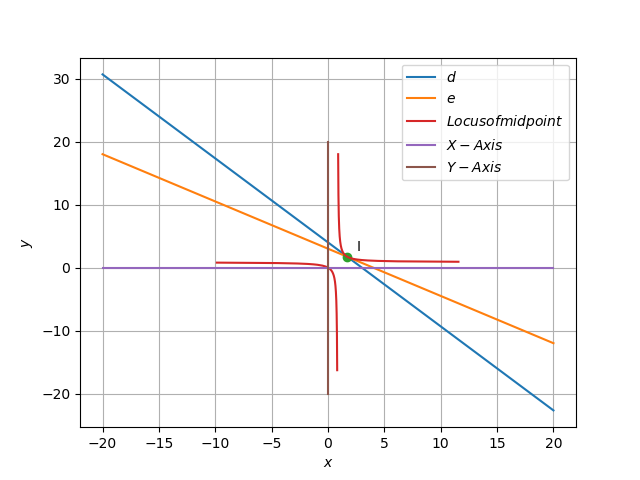
\includegraphics[scale=0.5]{locus}
\caption{locus diagram}
\end{figure}

\end{frame}
\begin{frame}
The figure of variable lines
\begin{figure}
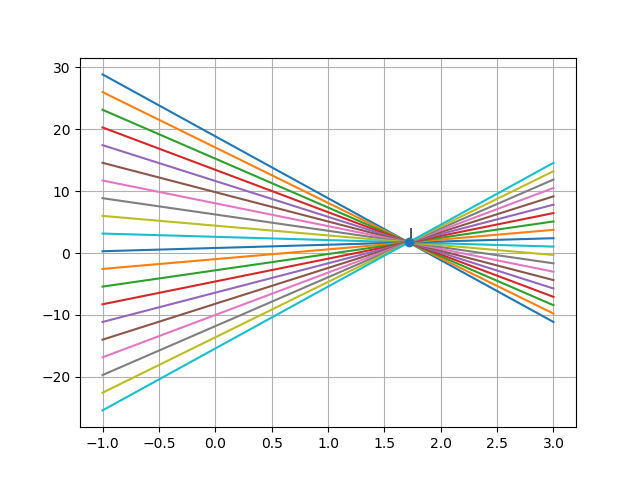
\includegraphics[scale=0.5]{variable_lines}
\caption{variable lines}
\end{figure}

\end{frame}
\begin{frame}
The figure of a random line among variable lines and line joining origin and X
\begin{figure}
\includegraphics[scale=0.5]{randomlinne}
\end{figure}
\end{frame}
\end{document}




